\section{Algoritmo}

\subsection{Busqueda Vectorial}

Suponiendo que tenemos un conjunto de \(n\) vectores \(V \in R^D\), donde \(D\) 
es la dimensi\'on de un vector. Realizar una busqueda vectorial 
\(\operatorname{NN}(x)\) en \(V\) se define\footnote{
    Esta es la definici\'on dada en \cite{pqnns}.}: 

\begin{align}
    \operatorname*{NN}(x) &= \operatorname*{argmin}_{y \in V} d(x, y)
\end{align}

D\'onde \(d(x,y)\) es la funci\'on de distancia entre dos vectores.
Por ende \(\operatorname{NN(x)}\) se puede describir como encontrar el vector 
m\'as cercano a \(x\) en \(V\). 

Una implementaci\'on basica de esto se puede ver as\'i: 

\begin{lstlisting}[language=C, caption=Algoritmo sin PQ]
float *NN(float *V, int n, float *x) {
    float *result;
    float min_dist = MAX;
    for (int i = 0; i < n; i++) {
        float *y = get_vector(V, i);
        float dist = d(x, y);
        if (dist < min_dist) {
            min_dist = dist; 
            result = y;
        }
    }

    return result;
}
\end{lstlisting}

Uno de los problemas principales de esta soluci\'on es que requiere que todos 
los vectores \(V\) esten guardados en memoria para realizar la busqueda. 
Este problema es el que se soluciona con PQ.

\newpage
\subsection{Cuantificaci\'on de Productos (PQ)}

PQ codifica los vectores en multiples indices a tablas de busqueda, 
comprimiendo su tama\~no, pero perdiendo los vectores originales (compresion 
con perdida). 

Los vectores primero se separan en \(m\) subvectores, \(m\) siendo un multiplo
de \(D\). Llamamos \(D'\) a la dimensi\'on de un subvector, y \(S\) a los
conjuntos de subvectores tal que:
\begin{align}
  S_i &= \{ x_{D'i+1}, x_{D'i+2}, \dots, x_{D'(i+1)} \} 
  \hspace{5pt} 
  \forall i \in [1,m]
\end{align}

Y lo podemos visualizar en \ref{fig:subvectores}.

\begin{figure}[ht]
\begin{tikzpicture}
  [
    2d-arr/.style={
      matrix of nodes,
      nodes in empty cells,
      row sep=-\pgflinewidth,
      column sep=-\pgflinewidth,
      align=center,
      nodes={
        draw,
        minimum height=25pt,
        text width=50pt,
        align=center,
        anchor=center,
        outer sep=0pt,
      }
    },
    teal-thick/.style={
      ultra thick,
      inner sep=0.5pt,
      rounded corners=1mm,
      draw=teal
    },
  ]

  \matrix(vectors)[
    2d-arr,
    right delimiter=\},
    row 3/.style={nodes={draw=none}},
    column 4/.style={nodes={fill=teal!30}},
  ] { % use \& instead of & as column separator
    $s_{1,1}$ & $s_{1,2}$ & \tiny{\dots} & $s_{1,i}$ & \tiny{\dots} & $s_{1,m-1}$ & $s_{1,m}$ \\
    $s_{2,1}$ & $s_{2,2}$ & \tiny{\dots} & $s_{2,i}$ & \tiny{\dots} & $s_{2,m-1}$ & $s_{2,m}$ \\
    & & & \tiny{\vdots} & & & \\
    $s_{n,2}$ & $s_{n,2}$ & \tiny{\dots} & $s_{n,i}$ & \tiny{\dots} & $s_{n,m-1}$ & $s_{n,m}$ \\
  };

  \node [outer sep=10pt, right] at(vectors.east) {$n$};
  \node [left, overlay] at(vectors.west) {$V =$};

  % \draw (vectors-1-4.north west) rectangle (vectors-4-4.south east);
  \matrix(subvectors)[
    2d-arr,
    right delimiter=\},
    nodes={
      fill={teal!30}
    },
  ] at (0, -4) { % use \& instead of & as column separator
    $x'_{1,1}$ & $x'_{1,2}$ & \tiny{\dots} & $x'_{1,D'}$ \\
    $x'_{2,1}$ & $x'_{2,2}$ & \tiny{\dots} & $x'_{2,D'}$ \\
    & & & \\
    $x'_{n,1}$ & $x'_{n,2}$ & \tiny{\dots} & $x'_{n,D'}$ \\
  };

  \node [outer sep=10pt, right] at(subvectors.east) {$n$};

  \node(bounding)[
    fit={(vectors-1-4.north west) (vectors-4-4.south east)},
    teal-thick
  ]{};

  \node(bounding)[
    fit={(subvectors-4-4.south east) (subvectors-1-1.north west)},
    teal-thick,
    label={[align=right]180:$S_i= $}
  ]{};

  \draw[teal-thick] {
    (vectors-4-4.south west) -- (subvectors-1-1.north west)
    (vectors-4-4.south east) -- (subvectors-1-4.north east)
    (vectors-4-4.south east) -- (vectors-4-4.south west)
  };
  \useasboundingbox (0,1.5);


\end{tikzpicture}

\caption{Subvectores en $V$}
\label{fig:subvectores}
\end{figure}

Para cada \(S_i\), calculamos \(k\) centroides usando el algor\'itmo de 
clustering K-means \cite{wiki:K-means_clustering}. 
Llamaremos a estos centroides \(C_i\). 
Un ejemplo del resultado de este algoritmo se puede ver visualmente en 
\ref{fig:kmeans-ej}.

\newpage 

Una vez que tenemos estos centroides, podemos codificar los subvectores a sus 
centorides m\'as cercanos definiendo: 
\begin{align}
  q_i(s) &= \operatorname*{argmin}_{c \in C_i} d(s, c) 
\end{align}

Y aplicandolo a todo \(S_i\): 
\begin{align}
  s &\rightarrow q_i(s') \forall s \in S_i
\end{align}
Lo cual podemos ver en \ref{fig:centroids}

\begin{figure}
\centering
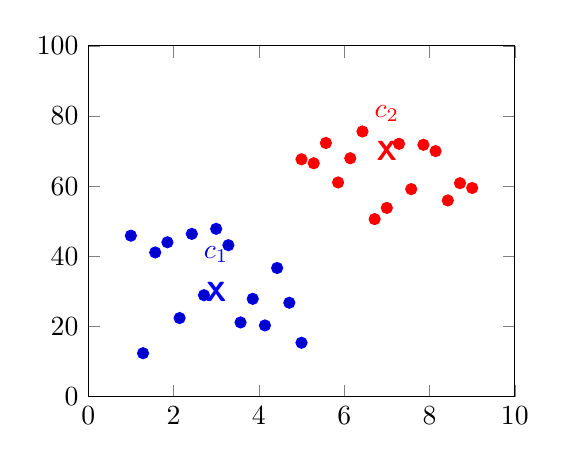
\begin{tikzpicture}
  \begin{axis}[
        width=7cm,
        xmin=0,xmax=10,ymin=0,ymax=100,
        ]
       \node[
         text=blue,
         font=\sffamily\bfseries,
         scale=1,
         label={[text=blue]$c_1$}
       ] at (3,30) {X};
       \addplot+[y filter/.expression={y+10},only marks,mark=*,samples=15,domain=1:5] {40*rnd};

       \node[
         text=red,
         font=\sffamily\bfseries,
         scale=1,
         label={[text=red]$c_2$}
       ] at (7,70) {X};
       \addplot+[y filter/.expression={y+50},only marks,mark=*,mark options={fill=red},samples=15,domain=5:9] {40*rnd};
  \end{axis}
\end{tikzpicture}

\caption{Ejemplo K-Means ($k=2$, $D'=2$)}
\label{fig:kmeans-ej}
\end{figure}

\begin{figure}[h]
\centering
  \begin{tikzpicture}
    [
      % transform shape,
      2d-arr/.style={
        matrix of nodes,
        nodes in empty cells,
        row sep=-\pgflinewidth,
        column sep=-\pgflinewidth,
        align=center,
        nodes={
          draw,
          minimum height=20pt,
          text width=40pt,
          align=center,
          anchor=center,
          outer sep=0pt,
        }
      },
      teal-thick/.style={
        ultra thick,
        inner sep=0.5pt,
        rounded corners=1mm,
        draw=teal
      },
      matrix/inner style order={
        every cell,
        even odd column,
        column, 
        even odd row,
        row,
        cell
      }
    ]

    \matrix(vectors)[
      2d-arr,
      right delimiter=\},
      row 3/.style={nodes={draw=none}},
      every even column/.style={nodes={fill=teal!30}},
      column 1/.style={nodes={fill=teal!50}},
      column 7/.style={nodes={fill=teal!50}},
    ] { % use \& instead of & as column separator
      $s_{1,1}$ & $s_{1,2}$ & \tiny{\dots} & $s_{1,i}$ & \tiny{\dots} & $s_{1,m}$ \\
      $s_{2,1}$ & $s_{2,2}$ & \tiny{\dots} & $s_{2,i}$ & \tiny{\dots} & $s_{2,m}$ \\
      & & & \tiny{\vdots} & & \\
      $s_{n,1}$ & $s_{n,2}$ & \tiny{\dots} & $s_{n,i}$ & \tiny{\dots} & $s_{n,m}$ \\
    };

    \node [outer sep=10pt, right, overlay] at(vectors.east) {$n$};
    \node [left, overlay] at(vectors.west) {$V =$};

    \matrix(centroids)[
      2d-arr,
      below,
      row 4/.style={nodes={draw=none}},
      % row 1/.style={nodes={fill=black!20}},
      column 3/.style={nodes={draw=none, fill=none}},
      column 4/.style={nodes={fill=orange!50}},
      column 5/.style={nodes={draw=none, fill=none}},
      every odd column/.style={nodes={fill=orange!50}},
      every even column/.style={nodes={fill=orange!30}},
      row 1/.style={nodes={draw=none, fill=none}},
      column sep=10pt,
    ] at($ (vectors.south) - (0, 0.5) $) {
      $C_1$ & $C_2$ & \tiny{\dots} & $C_i$ & \tiny{\dots} & $C_m$ \\
      $c_{1,1}$ & $c_{1,2}$ & \tiny{\dots} & $c_{1,i}$ & \tiny{\dots} & $c_{1,m}$ \\
      $c_{2,1}$ & $c_{2,2}$ & \tiny{\dots} & $c_{2,i}$ & \tiny{\dots} & $c_{2,m}$ \\
      \tiny{\vdots} & \tiny{\vdots} & & \tiny{\vdots} & & \tiny{\vdots} \\
      $c_{k,1}$ & $c_{k,2}$ & \tiny{\dots} & $c_{k,i}$ & \tiny{\dots} & $c_{k,m}$ \\
    };

    \matrix(centroids-empty)[
      2d-arr,
      above left,
      nodes={style={draw=none, fill=none}},
      column sep=10pt,
      right delimiter=\},
    ] at($ (centroids.south east) $) {
      \\
      \\
      \vdots \\
      \\
    };

    \node [outer sep=10pt, right, overlay] at(centroids-empty.east) {$m$};

    \foreach \i in {1,...,6} {
      \ifthenelse{\i=3 \OR \i=5} {
      }{
        \draw[very thick, -stealth, orange] (vectors-4-\i) -- (centroids-1-\i);
      }
    }

    \node[overlay, align=center, font=\small\itshape, fill=orange!40]
    at ($(vectors-4-3)!0.5!(centroids-1-3)$) 
    {K-Means};

    \matrix(vectors-quantized)[
      2d-arr,
      below,
      row 3/.style={nodes={draw=none}},
      column 3/.style={nodes={fill=none}},
      column 4/.style={nodes={fill=purple!50}},
      column 5/.style={nodes={fill=none}},
      every odd column/.style={nodes={fill=purple!50}},
      every even column/.style={nodes={fill=purple!30}},
      nodes={font=\scriptsize},
      right delimiter=\},
    ] at($ (centroids.south) - (0, 0.5) $) {
      $q_1(s_{1,1})$ & $q_2(s_{1,2})$ & \tiny{\dots} & $q_i(s_{1,i})$ & \tiny{\dots} & $q_m(s_{1,m})$ \\
      $q_1(s_{2,1})$ & $q_2(s_{2,2})$ & \tiny{\dots} & $q_i(s_{2,i})$ & \tiny{\dots} & $q_m(s_{2,m})$ \\
      & & & \tiny{\vdots} & & \\
      $q_1(s_{n,1})$ & $q_2(s_{n,2})$ & \tiny{\dots} & $q_i(s_{n,i})$ & \tiny{\dots} & $q_m(s_{n,m})$ \\
    };

    \node [outer sep=10pt, right, overlay] at(vectors-quantized.east) {$n$};

    \foreach \i in {1,...,6} {
      \ifthenelse{\i=3 \OR \i=5} {
      }{
        \draw[very thick, -stealth, purple] 
          (centroids-5-\i) -- (vectors-quantized-1-\i);
      }
    }

    \node[overlay, align=center, font=\small\itshape, fill=purple!40]
    at ($(centroids-5-3)!0.5!(vectors-quantized-1-3)$) 
    {$q_i(x)$};

    \node[left, align=center, overlay] at(vectors-quantized.west) 
      {\(V\) \\ Cuantificado};

  \end{tikzpicture}
\caption{Vectores cuantificados.}
\label{fig:centroids}
\end{figure}

\newpage

Finalmente, en vez de usar \(q_i(s)\) para codificar a \(s\), podemos usar el 
\'indice de \(q_i(s)\) en \(C_i\), comprimiendo el tama\~no de los vectores.

\subsection{Busqueda con PQ}

Hasta ahora con el algoritmo podemos entrenar y agregar los vectores al espacio 
de busqueda. 
Para realizar la busqueda, hacemos un calculo de distancia asim\'etrico 
(ADC en \cite{pqnns}), donde el vector de b\'usqueda \(v\) no se cuantifica con 
PQ, sino que se calcula directamente la distancia con los vectores 
decodificados.

Dado esto, retornamos los \(k\) vecinos mas cercanos (a no confundir con los 
\(k\) centroides por subespacio) al vector de busqueda. 

